\documentclass{article}
\usepackage[T1]{fontenc}
\usepackage{lmodern}
\usepackage{graphicx}
\usepackage{amsmath,amssymb}
\usepackage[a4paper,margin=2cm]{geometry}
\usepackage[absolute,overlay]{textpos}
\setlength{\TPHorizModule}{1mm}
\setlength{\TPVertModule}{1mm}
\usepackage[indonesian]{babel}
\usepackage{hyperref}
\setlength{\emergencystretch}{2em}
% unit: Halaman 9

\begin{document}

% === Halaman 9 (llm) ===

\begin{itemize}
    \item Algoritma pertukaran kunci Diffie-Hellman dipublikasikan oleh Whitfield Diffie dan Martin Hellman pada tahun 1976
\end{itemize}

\vspace{50mm}

Whitfield \textbf{Diffie} dan Martin \textbf{Hellman}

\vspace{10mm}
Rinaldi M/II4020 Kriptografi

% deskripsi: Foto potret Whitfield Diffie dan Martin Hellman berdampingan
% bbox normalisasi: [0.2400, 0.3100, 0.6920, 0.8110]
\begin{textblock*}{94.92mm}(50.40mm,92.07mm)
\noindent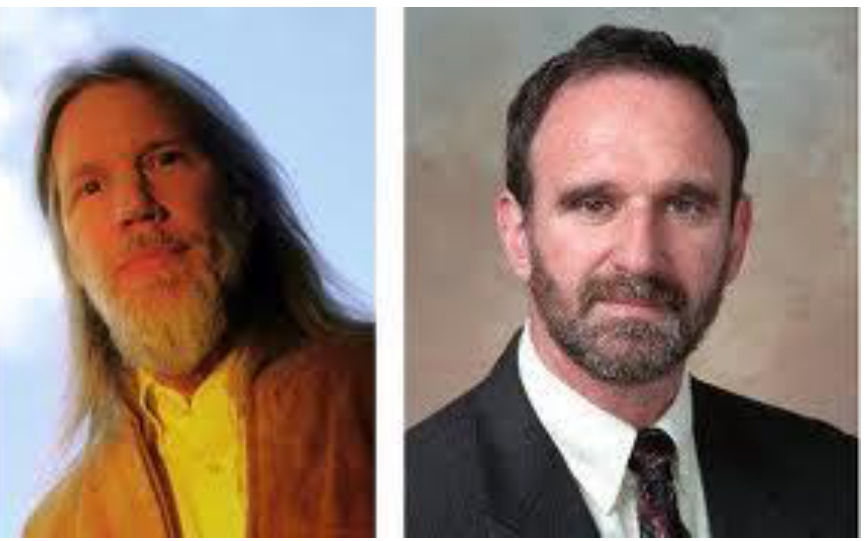
\includegraphics[width=94.92mm,height=148.80mm]{../../images/llm/page_009_img_01.png}%
\end{textblock*}

\end{document}
